\chapter{Background}

\section{What is eBPF?}

\textbf{eBPF} (extended Berkeley Packet Filter) is a \textbf{revolutionary in-kernel virtual machine} that allows user-supplied programs to execute safely within the Linux kernel. It evolved from classic BPF (1992, used for packet filtering in \texttt{tcpdump}) and became a \textbf{general-purpose sandboxed execution environment} in Linux 3.18 (2014).

\noindent
eBPF provides a complete execution environment featuring 11 registers and a 64-bit word size, supporting key-value stores called Maps for inter-program and user-space communication. The architecture includes Helpers, which are kernel function calls with specific signatures, allowing eBPF programs to interact with the kernel in controlled ways. Hooks provide attachment points throughout the kernel stack, including kprobes for function instrumentation, tracepoints for static kernel events, XDP for network packet processing, TC for traffic control, and LSM for security policies. Finally, JIT compilation translates eBPF bytecode directly into native CPU instructions, enabling near-native performance.

\noindent
eBPF has become ubiquitous in modern Linux deployments. Observability platforms like Cilium and Falco use eBPF for real-time system monitoring. Networking companies such as Calico and Cloudflare leverage it for advanced packet processing. Security applications employ eBPF for runtime threat detection, policy enforcement, and Linux Security Module integration.

\begin{figure}[h]
\centering
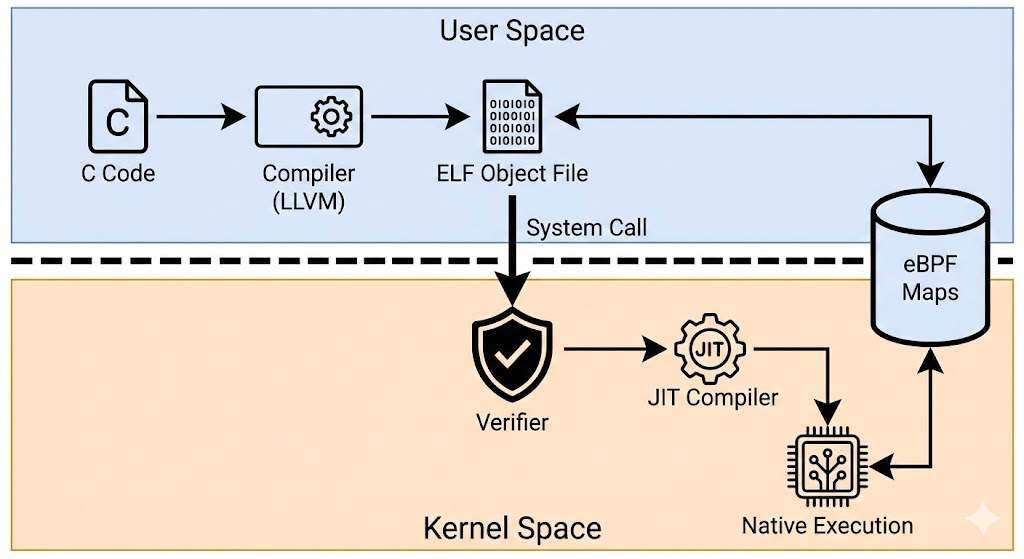
\includegraphics[width=0.7\textwidth]{resources/images/ebpf_architecture.jpg}
\caption{eBPF Architecture Overview: The complete execution pipeline from user-space through the kernel}
\end{figure}

\section{The eBPF Verifier: Security Cornerstone}

The verifier is a \textbf{static analyzer} that runs before every eBPF program is executed. Its primary responsibility is to guarantee four critical security properties: \textbf{memory safety} (preventing out-of-bounds reads and writes), \textbf{termination} (ensuring all code paths complete with bounded loops), \textbf{type safety} (enforcing correct use of pointers and scalar types), and \textbf{helper compliance} (validating that kernel function arguments match expected types and counts).

\subsection{Verifier Operation}

The verifier's operation follows a sophisticated simulation strategy. It constructs a control-flow graph of the program, then simulates execution along each path, maintaining state for all 11 registers. For each register, the verifier tracks three key properties: its type (whether it holds a SCALAR number or a POINTER to memory or maps), its range or value bounds represented internally as a \texttt{tnum} in kernel code, and for pointers, the offset relative to the base object. A vulnerability occurs precisely when the verifier's internal state model diverges from the actual runtime machine state, allowing unsafe operations to slip past verification.

\subsection{Verifier Limitations and Attack Surface}

The verifier is extraordinarily \textbf{complex}, comprising approximately 20,000 lines in \textbf{kernel/bpf/verifier.c}, and operates under tight performance constraints to avoid slowing down program loading. This complexity and the need for performance create potential for \textbf{logic bugs} in several categories.

\noindent
\textbf{Pruning failures} occur when the verifier skips re-verification of code paths it deems ``similar'' to previously verified paths, but which are actually unsafe. \textbf{Type confusion} happens when the verifier incorrectly tracks whether a register holds a SCALAR or a POINTER, leading to unsafe memory access. \textbf{Bounds propagation errors} cause the verifier to lose track of arithmetic constraints as operations compose, allowing values to exceed their documented ranges. \textbf{ABI assumption errors} (ABI = Application Binary Interface) arise from misunderstandings about how function calls marshal arguments across the verifier boundary, particularly when dealing with function pointers.

\noindent
The real-world impact of such verifier bugs is significant. Historical CVEs in eBPF's verifier include CVE-2020-8835 (enabling arbitrary read/write), CVE-2021-3490 (ALU32 bounds tracking error), CVE-2022-23222 (pointer arithmetic confusion), and CVE-2023-2163 (verifier log buffer overflow). Each of these represents a case where carefully crafted eBPF code bypassed the verifier's safety checks and reached kernel execution.

\section{The XDP SynProxy Target}

\subsection{Why XDP?}

\begin{figure}[h]
\centering
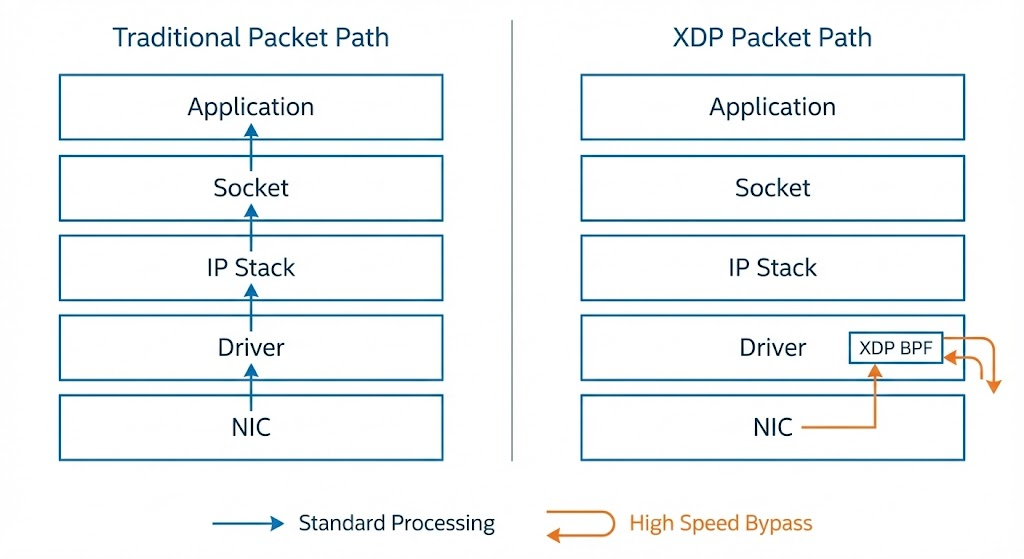
\includegraphics[width=0.7\textwidth]{resources/images/xdp_stack_comparison.jpg}
\caption{XDP Processing: Earliest point in the network stack before traditional TCP/IP processing}
\end{figure}

\noindent
\textbf{XDP (eXpress Data Path)} is a hook point at the network driver level, executing before packets enter the kernel's normal networking stack. This location is ideal for security research for several reasons. First, it processes packets at the earliest possible point in the stack, enabling line-rate packet processing without the overhead of traditional kernel networking code. Second, XDP programs have direct access to packet buffers without indirection, allowing efficient memory manipulation. Third, real-world XDP code performs complex pointer arithmetic on network headers (Ethernet, IP, TCP), creating opportunities for the kind of parsing vulnerabilities we study. Finally, XDP is critical infrastructure for DDoS mitigation, firewall rules, and load balancing, making verifier bugs here particularly impactful.

\subsection{SYN Proxy Fundamentals}

\noindent
A SYN Proxy solves a fundamental problem in network security: defending against SYN flood attacks. These attacks exploit the TCP three-way handshake by sending thousands of SYN packets with spoofed source addresses, exhausting server connection tables without ever completing the handshake. A SYN Proxy intercepts these packets and validates clients before allowing real connections to the server, using cryptographic SYN cookies to track state without storing per-connection data.

\begin{figure}[h]
\centering
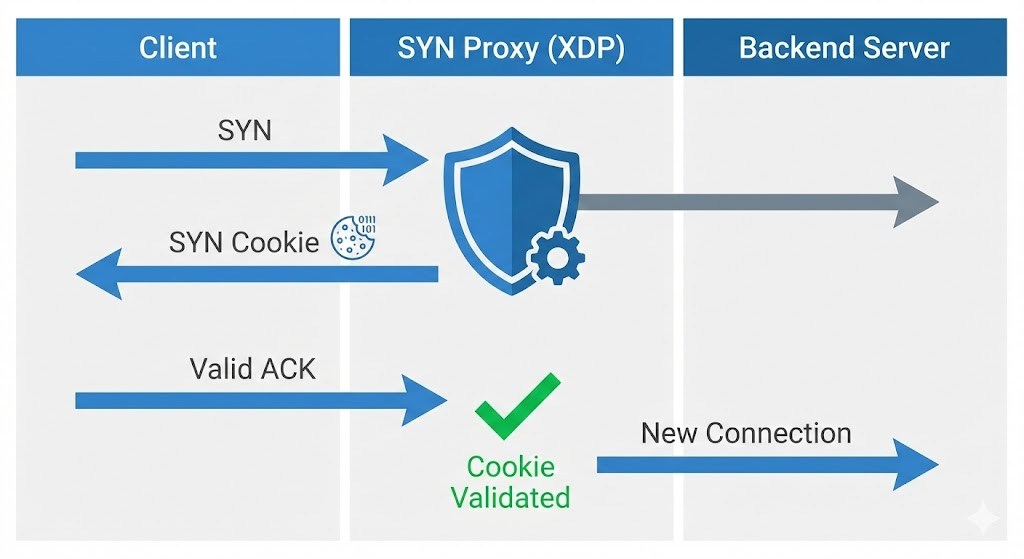
\includegraphics[width=0.7\textwidth]{resources/images/syn_proxy_flow.jpg}
\caption{SYN Proxy Flow: Intercepting and validating client connections}
\end{figure}

\noindent
The XDP SynProxy in the Linux selftests (\texttt{xdp\_synproxy\_kern.c}) implements this defense directly at the driver level. When a SYN packet arrives, the program parses Ethernet, IP, and TCP headers to identify the connection parameters. For incoming SYN packets, it generates a cryptographic SYN cookie encoding the client's address, port, and timestamp, then crafts a SYN-ACK response containing this cookie as the sequence number. When the client returns with an ACK containing the cookie, the program validates the cookie and, if correct, allows the connection through. This implementation uses complex pointer arithmetic for header parsing, eBPF maps for state management, and multiple kernel helper functions, making it an excellent target for testing whether the verifier correctly handles real-world eBPF code.

\section{The Prior Team's Work}

\subsection{ISO-IEC TS 17961-2013 Rule-Based Assessment}

A previous team (Francesco Rollo, Gianfranco Trad, Giorgio Fardo, Giovanni Nicosia) systematically applied each of the 46 rules from ISO-IEC TS 17961-2013 (C Secure Coding Standard) to the XDP SynProxy program. For each rule, they asked: \textit{``If we intentionally violate this rule in the eBPF code, does the verifier catch it?''}

\noindent
The assessment found:
\begin{itemize}
  \item \textbf{22 rules not applicable}: No dynamic memory allocation, signals, or file I/O in eBPF
  \item \textbf{24 rules testable}: Applied within eBPF's architecture constraints
  \item \textbf{21 violations passed the verifier}: A concerning finding that motivated this practical follow-up
\end{itemize}

\subsection{Classification of Findings}

The prior team classified each violation into outcomes:
\begin{table}[h]
\centering
\begin{tabular}{|l|c|l|}
\hline
\textbf{Outcome} & \textbf{Count} & \textbf{Interpretation} \\
\hline
Verifier blocked & 14 & Security working correctly \\
Compiler optimized away & 8 & Never reached verifier \\
Verifier passed + Exploitable & 9 & \textbf{CRITICAL} \\
Verifier passed + Limited & 12 & Uncertain exploitation potential \\
Verifier passed + Safe & 17 & Logic bugs without security impact \\
\hline
\end{tabular}
\caption{Classification of 60+ rule violations tested against verifier}
\end{table}

\section{The Theory-to-Practice Gap}

\textbf{Critical insight}: Knowing a vulnerability \textit{passes the verifier} is not the same as knowing it is \textit{actually exploitable}.

\subsection{The Translation Chain}

An eBPF exploit must survive multiple translation stages:
\begin{enumerate}[label=\arabic*.]
  \item \textbf{C source code}: Developer writes vulnerability
  \item \textbf{LLVM compilation}: Translates to eBPF bytecode (may optimize away the bug)
  \item \textbf{eBPF verifier}: Accepts or rejects the program
  \item \textbf{JIT compilation}: Translates bytecode to native machine code (x86/ARM)
  \item \textbf{Runtime execution}: The actual vulnerability is triggered
\end{enumerate}

\noindent
At any stage, the vulnerability can be neutralized:
\begin{itemize}
  \item LLVM may dead-code-eliminate a branch
  \item eBPF's memory model (512-byte stack, 64-bit registers) may force safe translation
  \item The runtime verifier may reject or transform unsafe operations
\end{itemize}

\noindent
\textbf{Implication}: This work must analyze the bytecode produced, not just the C source code, to confirm vulnerabilities survive compilation.
